%%%%%%%%%%%%%%%%%%%%%%%%%%%%%%%%%%%%%%%%%%%%%%%%%%%%%%%%%%%%%%%%%%%%%%%%%%%%%%%%%%
\begin{frame}[fragile]\frametitle{}
\begin{center}
{\Large Conclusions}
\end{center}
\end{frame}

%%%%%%%%%%%%%%%%%%%%%%%%%%%%%%%%%%%%%%%%%%%%%%%%%%%%%%%%%%%
\begin{frame}[fragile]\frametitle{Challenges in Standard RAG}
    \begin{itemize}
        \item \textbf{Lack of Explainability:} Hard to trace the source of retrieved information.
        \item \textbf{Local Window:} Limited chunk-level context leads to incomplete responses.
        \item \textbf{Scalability Issues:} Struggles with large-scale medical and legal corpora.
        \item \textbf{Loss of Structural Relationships:} Ignores hierarchical relationships in data.
    \end{itemize}
\end{frame}


%%%%%%%%%%%%%%%%%%%%%%%%%%%%%%%%%%%%%%%%%%%%%%%%%%%%%%%%%%%
\begin{frame}[fragile]\frametitle{}

	\begin{center}
	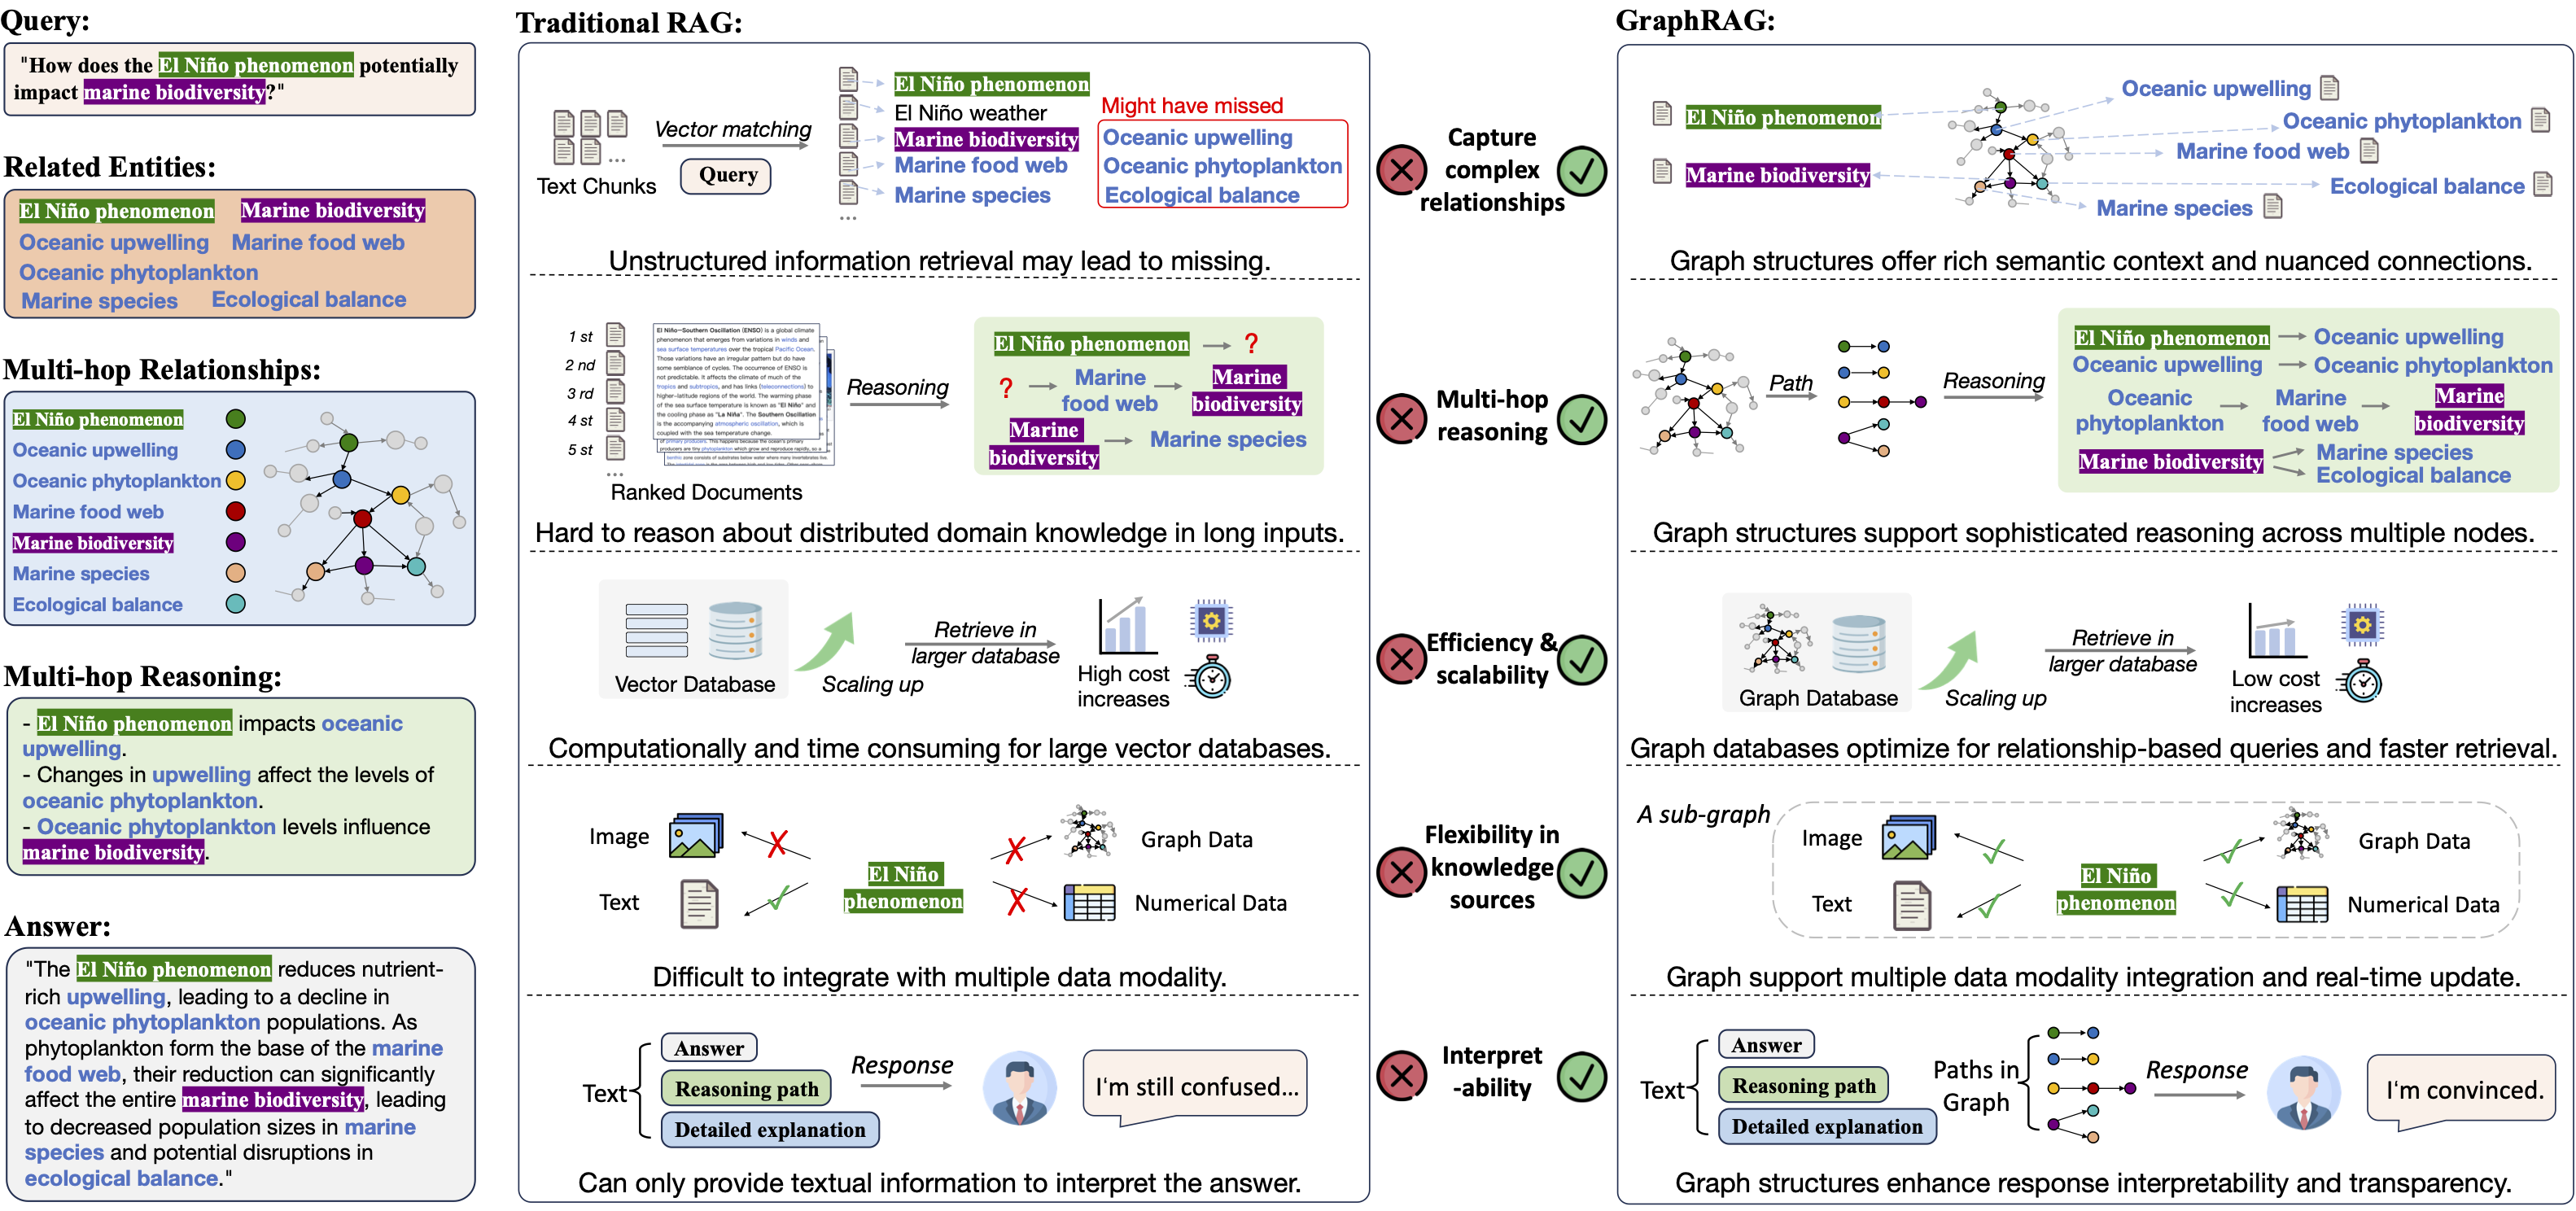
\includegraphics[width=\linewidth,keepaspectratio]{rag_vs_graphrag}
	\end{center}
	
\end{frame}


%%%%%%%%%%%%%%%%%%%%%%%%%%%%%%%%%%%%%%%%%%%%%%%%%%%%%%%%%%%
\begin{frame}[fragile]\frametitle{Key Features of GraphRAG}
    \begin{itemize}
        \item \textbf{Structured Representation:} Uses knowledge graphs.
        \item \textbf{Contextual Retrieval:} Understands semantic relationships.
        \item \textbf{Efficient Processing:} Reduces computational cost.
        \item \textbf{Multi-Faceted Queries:} Synthesizes data from multiple sources.
        \item \textbf{Explainability:} More transparent than black-box models.
        \item \textbf{Continuous Learning:} Expands knowledge over time.
    \end{itemize}
\end{frame}

%%%%%%%%%%%%%%%%%%%%%%%%%%%%%%%%%%%%%%%%%%%%%%%%%%%%%%%%%%%
\begin{frame}[fragile]\frametitle{Different Approaches}

	\begin{table}[h!]
		\centering
			% \begin{tabular}{|p{3.5cm}|p{7cm}|p{5cm}|}	\hline
			\begin{tabular}{|l|p{4cm}|p{3.5cm}|}	\hline

			\textbf{Approach} & \textbf{Description} & \textbf{Key Differentiators} \\
			\hline
			Neo4j & LLM extracts entities, builds KG, translates queries to Cypher & Domain-specific entities + structured queries \\
			\hline
			LlamaIndex & Hierarchical graph + community detection + multi-level summaries & Layered context resolution \\
			\hline
			Microsoft & KG construction + Leiden clustering + community summaries & Dataset-wide insights \\
			\hline
			Hybrid & Vector search + graph traversal & Semantic + relational fusion \\
			\hline
			\end{tabular}
		% \caption{Key Approaches in Retrieval Augmented Generation on Graphs}
		% \label{tab:graphRAG_approaches}
	\end{table}

\end{frame}